\chapter{相变}
    \section{相变概念}
        关于相变,有一些最为基础的概念,
        \begin{enumerate}
            \item 相\index{相}:成分相同、结构相同,有界面同其他部分分隔的物质均匀组成部分;
            \item 相变\index{相变}:当外界条件(如温度、压力等)连续变化时,物质自身发生突变的现象。或物相的某个(阶)热力学势跃变,伴随物相的某个(些)要素跃变;
            \item 固态相变\index{固态相变}:固体材料的结构在温度、压力、成分改变时所发生的转变。
        \end{enumerate}

        在分类上,有很多种分类方法,比如从动力学上,或者是从热力学上分类
            \subsection{动力学相变分类}
                相变分为两类:扩散性和无扩散型,如\autoref{金属及合金中的一级相变}所示。
                无扩散型相变\index{无扩散型相变}较为简单,分为连续型相变\index{连续型相变},比如$\omega$相比\index{$\omega$相变},和形核长大型相变\index{形核长大型相变},比如马氏体相变\index{马氏体相变}。

                而扩散性相变\index{扩散性相变}则相对复杂,也分为连续型相变\index{连续型相变}和形核长大型相变\index{形核长大型相变},更为具体的分类将在后面的章节进行讲解,在这里不再进行过多叙述。
                \begin{figure}[ht]
                    \centering
                    \includegraphics[width=0.7\textwidth]{fig/first_phase_transformation_in_alloys.png}
                    \caption{金属及合金中的一级相变。}
                    \label{金属及合金中的一级相变}
                \end{figure}
            \subsection{热力学的相变分类}
                在热力学的分类比较简单,分为一级相变\index{一级相变}和二级相变\index{二级相变}。
                一级相变是指化学位相等,但是化学位的一阶导数不等,也就是熵不等或者是体积不等,
                \begin{align}
                    \mu_1&=\mu_2,\\
                    \left(  \frac{\partial\mu_1}{\partial T} \right)_p=-S_1&\neq-S_2= \left(  \frac{\partial\mu_2}{\partial T} \right)_p\label{等压一级相变},\\
                    \left(  \frac{\partial\mu_1}{\partial p} \right)_T=V_1&\neq V_2= \left(  \frac{\partial\mu_2}{\partial p} \right)_T\label{等温一级相变}.
                \end{align}
                在一级相变中伴有能量变化,或者吸热或者放热,或者体积发生变化。比如晶体的熔化、升华、液体的凝固、汽化、气体的凝聚以及晶体中大多数晶型转变都属于一级相变,这是最普遍的相变类型。

                二级相变是指化学位的二阶导数发生突变,而化学位和一阶导数不发生突变,
                \begin{align}
                    -\frac{C_p}{T}=\left(  \frac{ \partial^2\mu_1  }{\partial T^2} \right)_p&\neq\left(  \frac{ \partial^2\mu_2  }{\partial T^2} \right)_p,\\
                    kV=\left(  \frac{ \partial^2\mu_1  }{\partial p^2} \right)_T&\neq\left(  \frac{ \partial^2\mu_2  }{\partial p^2} \right)_T,\\
                    \alpha V=\frac{\partial^2\mu_1}{\partial T\partial p}&\neq\frac{\partial^2\mu_2}{\partial T\partial p}.
                \end{align}
                其中$C_p$为等压比热\index{等压比热},$k$为等温等压系数\index{等温等压系数},$\alpha$为等压膨胀系数\index{等压膨胀系数}\footnote{熔化、马氏体转变属一级相变,有序化可能是一级也
                可能是二级相变。}。
                在二级相变中,两相的化学势、熵和体积相等,但热容、膨胀系数和压缩系数不相等,即无相变潜热,无体积的突变,只有热容、
                膨胀系数和压缩系数的不连续变化,
                \begin{align*}
                    \Delta C_p\neq 0,\\
                    \Delta\beta\neq 0,\\
                    \Delta\alpha\neq0.\\
                \end{align*}
                一般合金的有序-无序转变、铁磁-顺磁转变、超导转变等属于二级相变。大多数便随某种物理性能的变化。
            \subsection{固溶体自由能的计算}
                纯组元的自由能和温度的关系可以写作
                \begin{equation}
                    G(T)=H(T)-TS(T),
                \end{equation}
                而两相混合的自由能,在理想条件下可以由两相的自由能叠加得到。

                假设在体系中存在两种相$\alpha$和$\beta$,均是由A、B两种原子构成,假设A原子的成分为$x\mathrm{at.}\%$,在$\alpha$相中,A的原子百分比为$x_1$,在$\beta$中的原子百分比为$x_2$
                而$\alpha$相和$\beta$的占比分别为$N_1$和$N_2$,两者的自由能分别为$G_1$和$G_2$,混合后的自由能为
                \begin{equation}
                    G=N_1G_1+N_2G_2,
                \end{equation}
                利用成分关系,可以变为
                \begin{equation}
                    G=G_1+\frac{x-x_1}{x_2-x_1}(G_2-G_1),
                \end{equation}
                所以$G_1$,$G$,$G_2$处于同一直线,并且服从杠杆定律。

                但是在混合过程存在其他作用,导致混合后的自由能不等于理想情况下的自由能。这里假设实际的自由能为
                \begin{equation}
                    G(x)=G^0+\Delta G^m,
                \end{equation}
                其中
                \begin{equation}
                    G^0=x_AG_A^0+x_BG_B^0,
                \end{equation}
                其中,$x_A$为$A$原子的原子百分比,$x_B$为$B$原子的原子百分比,而要计算$\Delta G^m$,需要先计算混合过程中的焓\index{焓}和熵\index{熵}的变化量。
                \subsubsection{混合过程中熵的改变量}
                    固态下的系统的熵主要由混合熵\index{熵!混合熵}(决定于原子可能排列的方式)和振动熵\index{熵!振动熵}(决定于温度和缺陷)组成,
                    混合熵的变化为
                    \begin{equation}
                        \Delta S^m=S_{AB}-(x_AS_A+x_BS_B),
                    \end{equation}
                    根据混合熵的定义
                    \begin{equation}
                        S=k\ln{\Omega},
                    \end{equation}
                    其中$k$为玻尔兹曼常数,$\Omega$为微观状态数,假设$A$的原子数为$N_A$,$B$的原子数为$N_B$,混合熵的变化为
                    \begin{equation}
                        \begin{split}
                        \Delta S^m&=S_{AB}-(x_AS_A+x_BS_B)\\
                        &=k\ln{\frac{N!}{N_A!(N-N_A)!}}-x_Ak \ln \left(C_{N_{A}}^{N_{A}}\right)  -x_Bk \ln \left(C_{N_{B}}^{N_{B}}\right)\\
                        &=k\ln{\frac{N!}{N_A!N_B!}}\\
                        &=k\left( \ln{N!}-\ln{N_A!}-\ln{N_B!} \right).                
                        \end{split}                                      
                    \end{equation}
                    根据Stirling公式,
                    \begin{equation}
                        \Delta S^m=-R(x_A\ln{x_A}+x_B\ln{x_B}),
                    \end{equation}
                    其中$R=kN$。
                \subsubsection{混合过程中焓的改变量}
                    接下来计算混合过程中焓的变化,利用溶液的准化学模型\index{准化学模型},假设
                    \begin{enumerate}
                        \item $A$,$B$两组元尺寸接近,排列无序;
                        \item 混合过程中体积基本不变,即$\Delta V=0$;
                        \item 原子只与最近邻的原子之间存在相互作用,即只计算最近邻原子之间的结合能。
                    \end{enumerate}
                    假设两个近邻原子之间额定结合能分别为$u_{AA}$、$u_{AB}$和$u_{BB}$,固溶体和组元的配位数均为$Z$。在恒压情况下,焓的改变仅与结合能的改变有关,
                    所以
                    \begin{align}
                        \text{混合前,}&u_{1}=\frac{1}{2} N_{A} Z u_{A A}+\frac{1}{2} N_{B} Z u_{B B},\\
                        \text{混合后,}&u_{2}=\frac{1}{2} N_{A} Z \frac{N_{A}}{N} u_{A A}+\frac{1}{2} N_{B} Z \frac{N_{B}}{N} u_{B B}+N_{A} Z \frac{N_{B}}{N} u_{A B}.
                    \end{align}
                    所以焓的变化量为
                    \begin{equation}
                        \Delta u^m=Z N\left(u_{A B}-\frac{u_{A A}+u_{B B}}{2}\right) x_{A} x_{B},
                    \end{equation}
                    令$\alpha'=ZN\left( u_{AB}-\frac{u_{AA}+u_{BB}}{2} \right)$,焓变可以写作
                    \begin{equation}
                        \Delta H^m=\alpha'x_Ax_B.
                    \end{equation}
            \subsection{混合过程的自由能改变量以及成分与自由能关系}
                所以混合过程中自由能随成分和温度变化的关系为
                \begin{equation}
                    G(x)=G_{A}^{0} x_{A}+G_{B}^{0} x_{B}+\alpha^{\prime} x_{A} x_{B}+R T\left(x_{A} \ln x_{A}+x_{B} \ln x_{B}\right)\label{混合过程的自由能曲线}.
                \end{equation}
                下面将对于这一曲线进行讨论。

                混合前的自由能为$G_{A}^{0} x_{A}+G_{B}^{0} x_{B}$为一条直线,而熵的改变量则由于成分百分比均小于1而小于0,但是$\alpha^{\prime}$,也就是原子结合能的改变量不是能够确定的事,需要分情况讨论。
                在此之前,先进一步确定曲线与成分的关系,
                \begin{align}
                    \frac{\partial G}{\partial x_{B}}&=-G_{A}^{0}+G_{B}^{0}+\alpha^{\prime}\left(x_{A}-x_{B}\right)+R T\left(\ln x_{B}-\ln x_{A}\right),\\
                    \frac{\partial^{2} G}{\partial x_{B}^{2}}&=-2 \alpha^{\prime}+R T\left(\frac{1}{x_{A}}+\frac{1}{x_{B}}\right).
                \end{align}
                由此可见,曲线中唯有成分也就是结合能的变化不能确定,下面将针对结合能变化的三种情况进行讨论。

                当原子结合能不发生改变时,也就是$\alpha^{\prime}=0$时,此时体系符合理想溶液模型,自由能的二阶导数
                \begin{equation}
                    \frac{\partial^{2} G}{\partial x_{B}^{2}}=R T\left(\frac{1}{x_{A}}+\frac{1}{x_{B}}\right)>0,
                \end{equation}
                $G(x)$为下垂线,及曲线的凹向朝上,如\autoref{混合时结合能不变的自由能曲线}所示。
                \input{fig/free_energy_curve.tex}

                当焓变小于零时,也就是$\Delta H^M<0$,
                \begin{equation}
                    \frac{\partial^{2} G}{\partial x_{B}^{2}}=2 \alpha^{\prime}+R T\left(\frac{1}{x_{A}}+\frac{1}{x_{B}}\right)<0,
                \end{equation}
                这时异类原子的结合力大于同类原子之间的结合力。表现为在溶解时会放出热量。此时$G(x)$为下垂线,曲线的凹陷更大,如\autoref{混合时结合能减小的自由能曲线}所示。

                当焓变大于零时,焓变与熵的变化为相反的作用,曲线的形状与两者的大小有关。
                
                
                \begin{figure}[ht]
    \centering
    %\begin{subfigure}[0.3\textwidth]
    \subfloat[$T>\frac{\alpha^{\prime}}{2R}$]
    {
        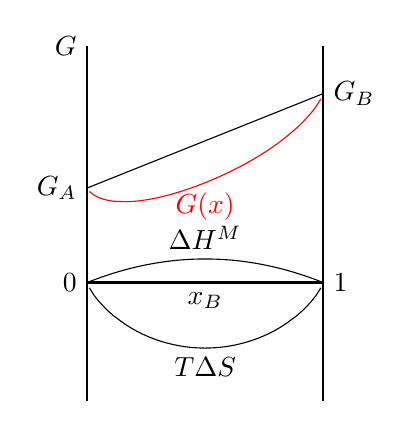
\begin{tikzpicture}[scale=3]
            \draw[thick] (0,0) node[anchor=east]{0} --(0.5,0) node[anchor=north] {$x_B$}--(1,0) node[anchor=west]{1};
            \draw[thick] (0,-0.5) -- (0,0.4) node[anchor=east]{$G_A$}--(0,1) node[anchor=east]{$G$};
            \draw[thick] (1,-0.5) -- (1,0.8) node[anchor=west]{$G_B$}--(1,1);
            
            \draw[thin] (0,0.4)--(1,0.8);
            \draw[domain=0.01:0.5] plot(\x,{0.4*(\x*ln(\x)+(1-\x)*ln((1-\x)))})
                node[below] {$T\Delta S$};
            \draw[domain=0.5:0.99] plot(\x,{0.4*(\x*ln(\x)+(1-\x)*ln((1-\x)))});
            
            %\Delta H
            \draw[domain=0:0.5] plot(\x,{0.4*(\x*(1-\x))})
                node[anchor=south] {$\Delta H^M$};
            \draw[domain=0.5:1] plot(\x,{0.4*(\x*(1-\x))});
            
            %G(x)
            \draw[red,domain=0.01:0.5] plot(\x,{0.4*\x+0.4+0.4*(\x*(1-\x))+0.4*(\x*ln(\x)+(1-\x)*ln((1-\x)))})
                node[below] {$G(x)$};
            \draw[red,domain=0.5:0.99] plot(\x,{0.4*\x+0.4+0.4*(\x*(1-\x))+0.4*(\x*ln(\x)+(1-\x)*ln((1-\x)))});        
        \end{tikzpicture}
       % \caption{$\Delta H^M=0$,混合时结合能不变的自由能曲线。}
        \label{subfig:高温下混合时结合能增加的自由能曲线}
    }
    
   % \end{subfigure}
   % \begin{subfigure}[0.3\textwidth]
    \subfloat[$0<T<\frac{\alpha^{\prime}}{2R}$]
    {
           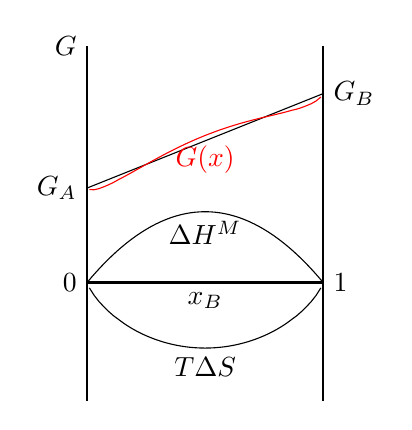
\begin{tikzpicture}[scale=3]
            \draw[thick] (0,0) node[anchor=east]{0} --(0.5,0) node[anchor=north] {$x_B$}--(1,0) node[anchor=west]{1};
            \draw[thick] (0,-0.5) -- (0,0.4) node[anchor=east]{$G_A$}--(0,1) node[anchor=east]{$G$};
            \draw[thick] (1,-0.5) -- (1,0.8) node[anchor=west]{$G_B$}--(1,1);
            %G(0)
            \draw[thin] (0,0.4)--(1,0.8);
            %T\Delta S
            \draw[domain=0.01:0.5] plot(\x,{0.4*(\x*ln(\x)+(1-\x)*ln((1-\x)))})
                node[below] {$T\Delta S$};
            \draw[domain=0.5:0.99] plot(\x,{0.4*(\x*ln(\x)+(1-\x)*ln((1-\x)))});
            %\Delta H
            \draw[domain=0:0.5] plot(\x,{1.2*(\x*(1-\x))})
                node[below] {$\Delta H^M$};
            \draw[domain=0.5:1] plot(\x,{1.2*(\x*(1-\x))});
            
            %G(x)
            \draw[red,domain=0.01:0.5] plot(\x,{0.4*\x+0.4+1.2*(\x*(1-\x))+0.4*(\x*ln(\x)+(1-\x)*ln((1-\x)))})
                node[below] {$G(x)$};
            \draw[red,domain=0.5:0.99] plot(\x,{0.4*\x+0.4+1.2*(\x*(1-\x))+0.4*(\x*ln(\x)+(1-\x)*ln((1-\x)))});        
        \end{tikzpicture}
        %\caption{$\Delta H^M<0$,混合时结合能小于零的自由能曲线。}
        \label{subfig:低温下混合时结合能增加的自由能曲线}
    }
    \subfloat[$T=0$]
    {
        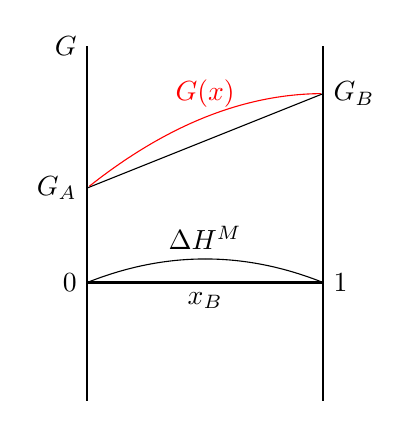
\begin{tikzpicture}[scale=3]
            \draw[thick] (0,0) node[anchor=east]{0} --(0.5,0) node[anchor=north] {$x_B$}--(1,0) node[anchor=west]{1};
            \draw[thick] (0,-0.5) -- (0,0.4) node[anchor=east]{$G_A$}--(0,1) node[anchor=east]{$G$};
            \draw[thick] (1,-0.5) -- (1,0.8) node[anchor=west]{$G_B$}--(1,1);
            %G(0)
            \draw[thin] (0,0.4)--(1,0.8);
            %T\Delta S
            %\draw[domain=0.01:0.5] plot(\x,{0.4*(\x*ln(\x)+(1-\x)*ln((1-\x)))})
            %    node[below] {$T\Delta S$};
            %\draw[domain=0.5:0.99] plot(\x,{0.4*(\x*ln(\x)+(1-\x)*ln((1-\x)))});
            %\Delta H
            \draw[domain=0:0.5] plot(\x,{0.4*(\x*(1-\x))})
                node[anchor=south] {$\Delta H^M$};
            \draw[domain=0.5:1] plot(\x,{0.4*(\x*(1-\x))});
            
            %G(x)
            \draw[red,domain=0.01:0.5] plot(\x,{0.4*\x+0.4+0.4*(\x*(1-\x))})
                node[anchor=south] {$G(x)$};
            \draw[red,domain=0.5:0.99] plot(\x,{0.4*\x+0.4+0.4*(\x*(1-\x))});        
        \end{tikzpicture}
        %\caption{$\Delta H^M<0$,混合时结合能小于零的自由能曲线。}
        \label{subfig:绝对零度下混合时结合能增加的自由能曲线}
    }
    %\end{subfigure}
    \caption{混合时结合能增加的在不同温度下的自由能曲线}

\end{figure}

                
                当$T\geq\frac{\alpha^{\prime}}{2R}$时,混合所提高的内能全部由热温熵来补充,$\Delta G^m\leq0$,曲线仍然为下垂曲线,仅仅是下垂的程度小一点,如\autoref{subfig:高温下混合时结合能增加的自由能曲线}所示。

                在低温情况下,$T<\frac{\alpha^{\prime}}{2R}$时,构成的曲线有三个极值点和两个拐点,在靠近坐标轴($x$接近0或1)处为上凹曲线,有两个极小值,而中部位凹向朝下的上凸曲线,会有一极大值,如\autoref{subfig:低温下混合时结合能增加的自由能曲线}所示。
                在这种情况下,存在两种必然的规律:
                \begin{enumerate}
                    \item[1] 任何一个组元都可以少量溶解其它组元,不可能得到绝对的纯净物质;
                    \item[2] 当出现上凸时,吉布斯自由能会提高,自发的趋势是形成两相混合物可以降低体系的自由能,两组元表现为有限溶解。
                \end{enumerate}
    \section{均匀形核}
        相变动力学\index{相变动力学}是讨论相变的过程和速度的,新相的形核\index{形核}和长大\index{长大}是动力学的两个基本问题。

        即使在宏观的单相均匀系统中,也存在着微观的不均匀性,存在局部的能量、密度、成分组态的涨落。Gibbs将这种涨落分为两类:
        \begin{enumerate}
            \item[1] 在\textbf{很小的体积}内存在着剧烈的原子再分布,在亚稳的母相中形成\textbf{新相胚芽},当这种胚芽超过临界尺寸\index{形核!临界尺寸},就变成稳定的新相核心而自发长大,金属和合金中的转变多数如此;
            \item[2] 在\textbf{大的体积内}原子的少量调整,\textbf{转变在整个体积范围内进行},如有序-无序转变\index{有序-无序转变}。
        \end{enumerate}

        以纯金属的凝固为例,假设在$L$中形成半径为$r$的晶核\index{形核!晶核}$s$,固体和液体的体积为$V_s$和$V_L$,固体和液体单位体积的自由能为$G_v^s$、$G_v^L$,$A_{SL}$为两相之间面积,$r_{SL}$为两相的界面能。

        假设发生相变的过程中没有体积变化,没有形核时,体系的自由能为
        \begin{equation}
            G_1=\left( V_s+V_l \right)G_v^L,
        \end{equation}
        则体系中出现晶核的自由能为:
        \begin{equation}
            G_2=V_sG_v^S+V_LG_v^L+A_{SL}\gamma_{SL},
        \end{equation}
        所以形核时的自由能变化为
        \begin{equation}
            \Delta G_v=G_2-G_1=-V_S\cdot \Delta G_v++A_{SL}\gamma_{SL},
        \end{equation}
        式中$\Delta G_v=G_v^L-G_v^S$。
        
        假设晶核为球形,则固液界面面积和固体体积为
        \begin{equation}
            A_{SL}=4\pi r^2, V=\frac{4}{3}\pi r^3,
        \end{equation}
        形核的自由能变化量为
        \begin{equation}
            \Delta G_r=-\frac{4}{3}\pi r^3\Delta G_v+4\pi r^2\gamma_{SL},
        \end{equation}
        在平衡状态下,对$r$求导,
        \begin{equation}
            \frac{\dif \Delta G_r }{\dif r}=-4\pi r^2\Delta G_v+8\pi r\gamma_{SL},
        \end{equation}
        令导数为零,此时的晶核半径为临界晶核尺寸\index{临界晶核尺寸}
        \begin{equation}
            r^*=\frac{\gamma_{SL}}{\Delta G_v}.
        \end{equation}
        自由能改变量为
        \begin{equation}
            \Delta G^*=\frac{16\pi}{3}\left( \frac{\gamma_{SL}^3}{\Delta G_v^2} \right),
        \end{equation}
        根据自由能的二阶导数可知,此时的自由能为极大值。因此只有半径大于临界晶核尺寸的晶核才能继续长大,而小于该尺寸的晶核则消失。
        临界晶核对于的自由能变化量$\Delta G^*$为形核功,即核长大到$r^*$所需克服的势垒。

        形核功的量值是临界球形晶核表面能的$1/3$,也就是说,球形晶核的表面能的$2/3$由新相的自由能下降给出,
        $1/3$依靠热涨落。这一过程称为\textbf{热激活过程}\index{形核!热激活过程}。

        在凝固过程中,要达到临界半径,需要温度上提供足够的过冷度,假设熔点温度为$T_m$,外界温度与熔点温度差为$\Delta T$,
        此时的自由能变化量为
        \begin{equation}
            \Delta G_v=\frac{\Delta T\cdot\Delta H_m}{T_m},
        \end{equation}
        代入临界半径表达式为
        \begin{equation}
            r^*=\frac{2\gamma_{LS}T_m}{\Delta H_m\cdot\Delta T},
        \end{equation}
        因此当$\Delta T=0$,$\Delta G^*\to0$,不能形核,过冷度越大,越易形核。
    \section{形核速率及均匀形核在固态转变中的推广}
        在液态的情况下,金属中也会存在一些小区域具有固态的密堆结构,本章将对这些小区域进行讨论。

        假设在单位体积内,由$i$个分子组成半径为$r$的胚芽数为$n_i$,而单分子数目为$n$,
        而单位体积中独立质点数$N$为
        \begin{equation}
            N=n+\sum_{i\geq2}n_i,
        \end{equation}
        由于$\sum_{i\geq2}n_i\ll n$,所以$N$约等于单位体积中的分子数。从统计方面考虑,胚芽数$n_i$服从玻尔兹曼分布:
        \begin{equation}
            n_i=N e^{-\frac{\Delta G_r}{kT}},
        \end{equation}
        临界核心数$n_i^*$为
        \begin{equation}
            n_i^*=N e^{-\frac{\Delta G_r^*}{kT}},
        \end{equation}
        其中$\Delta G_r^*$为形核功。

        在临界核心上痛殴分子碰撞再增加一个分子,它就可以克服势垒称为稳定的新相核心。
        定义单位体积中单位时间内形成的新相稳定核心的数目为形核速率\index{形核速率}$I$,
        所以形核速率$I$正比于临近核心的分子加入核心的频率$\omega$,即
        \begin{equation}
            I=\omega\cdot n_i^*=\omega N e^{-\frac{\Delta G_r^*}{kT}}\label{形核速率},
        \end{equation}
        $\omega$取决于原子振动频率、扩散激活能、晶核的表面积等。

        \subsection{形核引起的晶格畸变}
            在金属相变的过程中,由于晶核周围的体积和形状可能发生变
            化,或者晶核受到周围晶格的限制,使得晶核中的原子不能处
            在平衡位置,这两种情况都消耗弹性应变能$\varepsilon$,这种弹性应变
            能通过扩散和范性流变才能松弛。

            假定应变能正比于晶核的体积,则形核的自由能写作
            \begin{equation}
                \Delta G_r=-\frac{4}{3}\pi \cdot r^3(\Delta G_v+\varepsilon)+4\pi\cdot r^2\cdot\gamma_{SL},
            \end{equation}
            临界半径变为
            \begin{equation}
                r^*=\frac{2\gamma_{SL}}{\Delta G_v+\varepsilon},
            \end{equation}
            形核功为
            \begin{equation}
                \Delta G^*=\frac{16\pi \gamma^3_{SL}}{3(\Delta G_v+\varepsilon)^2}.
            \end{equation}
            另外,假设晶核的表面积对此时的邻近核心的分子加入核心的频率$\omega$没有影响,可以写为
            \begin{equation}
                \omega=ve^{-\frac{\Delta G_m}{kT}},
            \end{equation}
            其中$v$是原子振动频率\index{形核速率!原子振动频率},$\Delta G_m$是原子扩散的激活能\index{形核速率!扩散激活能}。所以\autoref{形核速率}可以写为
            \begin{equation}
                I=Nve^{-\frac{\Delta G^*+\Delta G_m}{kT}}\label{考虑外来扩散原子的形核速率},
            \end{equation}
            式中,$Nv$对$I$的影响很小,形核速率强烈依赖指数因子,也就是形核功和原子扩散激活能。
            对于固态相变,合理的数量级为
            \begin{equation*}
                Nve^{-\frac{\Delta G_m}{kT}}\simeq 10^{30},I=10^{30}e^{-\frac{\Delta G^*}{kT}}.
            \end{equation*}

            由于$\Delta G^*$因过冷度$\Delta T$的增大而减小,所以\textbf{形核速率强烈依赖于温度}。
            当$\Delta T\to0$,$\Delta G^*\to\infty$,$I\to0$,$\Delta T$增大,形核速率$I$存在极值,
            先增大后减小。

            \begin{figure}[ht]
                \centering
                    \subfloat[某合金的局部相图。]
                    {
                        \includegraphics{fig/nucleai_with_temperature/a.jpg}
                        \label{subfigure:某合金的局部相图}
                    }
                    \subfloat[相图的有效推动能量与形核功与转变温度之间的关系。]
                    {
                        \includegraphics{fig/nucleai_with_temperature/b.jpg}
                    }
                    \\
                    \subfloat[确定$I$的两个指数项与温度的关系。]
                    {
                        \includegraphics{fig/nucleai_with_temperature/c.jpg}
                    }
                    \subfloat[$I $随温度的变化。]
                    {
                        \includegraphics{fig/nucleai_with_temperature/d.jpg}
                        \label{subfigure:$I $随温度的变化}
                    }
                \caption{均匀形核速率$I$与转变温度之间的关系。}
                \label{均匀形核速率I与转变温度之间的关系}
            \end{figure}

            从\autoref{subfigure:某合金的局部相图}可知,成分为$x_0$的合金,其固溶温度为$T_e$,为了抵消应变能$\Delta G_\varepsilon$,
            必须过冷到$T_e^{\prime}$才能析出第二相$\beta$。形核速率随$T$的变化如\autoref{subfigure:$I $随温度的变化}所示,
            在高温下,沉淀的推动能量很小,因为$\Delta G^*$很大,所以$I$很小;在低温情况下,由于扩散很慢,所以$I$也很小,在中间某一个温度,
            $I$有极大值。

        \subsection{相界面性质的影响}

            界面能\index{界面能}$\gamma$的来源可以分为两部分,
            \begin{itemize}
                \item[1] 一部分是在母相中形成新相界面时,同类键和异类键的数量变化引起的,称为界面能中的\textbf{化学项}\index{界面能!化学项};
                \item[2] 另一部分是界面结构引起的 (如界面上产生的位错),称为界面能中的\textbf{结构项}\index{界面能!结构项}。
            \end{itemize}
            
            如果新相和母相的晶体结构和取向相同,电阵常数也非常接近,形成\textbf{完全共格界面}\index{完全共格界面}。界面能
            较小,只包括化学项,结构项(畸变能$\varepsilon$)趋于0,长大速度很快。

            如果完全共格两相的点阵常数不同,就会在界面上引入位错,来减少界面能中的体积应变能,结构项略有增大,形成\textbf{部分共格界面}\index{部分共格界面}。

            若新相通过母相切变形成,某些界面点阵相似,这种界面称为\textbf{切变共格}\index{切变共格}。

            如果所有界面都不共格,称为\textbf{非共格}\index{非共格}新相。

            
        \subsection{非均匀形核(界面形核)}
            形核过程若没有择优地点而称为均匀形核。实际上在金属或合金中,总是存在着界面、位错、夹杂等缺陷,因而
            成为非均匀的择优形核地点。主要是因为在缺陷处存在着畸变,在界面或缺陷处形核,可以消除缺陷,松弛部分能量,从而可以降低形核功。

            以锭模内表面的钢水凝固为例,在界面上形成球冠状的晶核,则有三种界面能$\gamma_{LS}$、$\gamma_{LC}$以及$\gamma_{SC}$,
            分别为液固界面能、液体锭模内壁界面能、固体锭模内壁界面能。达到平衡时,具有接触角,在水平上有
            \begin{equation}
                \gamma_{LC}=\gamma_{SC}+\gamma_{LS}\cos\theta\label{晶核形核过程中的力学平衡},
            \end{equation}
            这里不考虑$\gamma_{LS}$的垂直分量,它与锭模及晶核内聚力平衡,与此处无关系。

            假设晶核的曲率半径为$r$,晶核与锭模的接触面积为$A_1$,则
            \begin{equation}
                A_1=\pi\left( r\sin\theta \right)^2=\pi\cdot r^2\sin^2\theta,
            \end{equation}
            晶核与液体的接触面积为$A_2$,
            \begin{equation}
                A_2=2\pi\cdot r^2(1-\cos\theta),
            \end{equation}
            晶核的体积$V$为
            \begin{equation}
                V=\pi\cdot r^3\frac{2-3\cos\theta+\cos^3\theta}{3},
            \end{equation}
            形核之前,界面能为
            \begin{equation}
                \gamma_{LC}\cdot A_1=\gamma_{LC}\pi r^2\sin^2\theta,
            \end{equation}
            形核后,界面能为
            \begin{equation}
                \gamma_{LS}\cdot A_2+\gamma_{SC}\cdot A_1=\gamma_{LS}2\pi r^2(1-\cos\theta)+\gamma_{SC}\pi r^2\sin^2\theta,
            \end{equation}
            形核前后的界面能变化为
            \begin{equation}
                \begin{aligned}
                    \Delta G_s&=\gamma_{LS}\cdot A_2+\gamma_{SC}- \gamma_{LC}\cdot A_1\\
                    &=2 \pi \cdot r^{2}(1-\cos \theta)+\pi r^{2} \sin ^{2} \theta\left(\gamma_{s c}-\gamma_{L c}\right).
                \end{aligned}
            \end{equation}
            代入\autoref{晶核形核过程中的力学平衡}得到
            \begin{equation}
                \Delta G_{S}=\pi \cdot r^{2} \gamma_{L S}\left(2-3 \cos \theta+\cos ^{3} \theta\right).
            \end{equation}
            晶核形成时化学自由焓变化为
            \begin{equation}
                -V \cdot \Delta G_{v}=-\pi \cdot r^{3} \frac{2-3 \cos \theta+\cos ^{3} \theta}{3} \Delta G_{v},
            \end{equation}
            非均匀形核的自由能总改变量为上两项之和
            \begin{equation}
            \begin{aligned} 
                \Delta G_{\text{非}| \mathrm{E}} &=\Delta G_{s}+\left(-V \cdot \Delta G_{v}\right) \\ 
                &=\left(\pi \cdot r^{2} \cdot \gamma_{L S}-\frac{\pi \cdot r^{3}}{3} \cdot \Delta G_{v}\right) \cdot\left(2-3 \cos \theta+\cos ^{3} \theta\right) \\ 
                &=\left(-\frac{4 \pi \cdot r^{3}}{3} \Delta G_{v}+4 \pi \cdot r^{2} \gamma_{L S}\right). \cdot \frac{2-3 \cos \theta+\cos ^{3} \theta}{4} 
            \end{aligned}
            \end{equation}
            类似于前面求均匀形核功时的推导,平衡时有
            \begin{equation}
                \frac{\dif\left(\Delta G_{ \text{非}}\right)}{\dif r}=\left(-4 \pi \cdot r^{2} \cdot \Delta G_{v}+8 \pi \cdot r \cdot \gamma_{LS}\right) \cdot \frac{2-3 \cos \theta+\cos ^{3} \theta}{4}=0,
            \end{equation}
            此时临界半径为
            \begin{equation}
                r^*=\frac{2\gamma_{LS}}{\Delta G_v},
            \end{equation}
            对应的非均匀形核功为
            \begin{equation}
                \Delta G_{\text{非}}^{*}=\frac{16 \pi \gamma_{L S}^{3}}{3 \Delta G_{v}^{2}} \cdot \frac{2-3 \cos \theta+\cos ^{3} \theta}{4},
            \end{equation}
            对于均匀形核,形核功为
            \begin{equation}
                \Delta G^*_{\text{均}}\cdot\frac{2-3 \cos \theta+\cos ^{3} \theta}{4},
            \end{equation}
            由于
            \begin{equation}
                \frac{2-3 \cos \theta+\cos ^{3} \theta}{4}=\frac{(2+\cos \theta)(1-\cos \theta)^{2}}{4} \leq 1,
            \end{equation}
            所以,有以下结论:
            \begin{itemize}
                \item[1] $\theta=0$,$\cos\theta=1$,$\Delta G^*_{\text{非}}/\Delta G^*_{\text{均}}=0$,此时称为完全浸润;
                \item[2] $\theta=\frac{\pi}{2}$,$\cos\theta=0$,$\Delta G^*_{\text{非}}/\Delta G^*_{\text{均}}=\frac{1}{2}$;
                \item[3] $\theta=\pi$,$\cos\theta=-1$,$\Delta G^*_{\text{非}}/\Delta G^*_{\text{均}}=1$,此时称为完全不浸润;
                \item[4] 一般情况下,非均匀形核的形核功比均匀形核小。
            \end{itemize}
    
    \section{新相的长大}\label{section:新相的长大}
        在讨论完形核过程,接下来讨论相的长大过程。相长大有两种形式,分别为扩散型和非扩散型。
        其中扩散性又有两种分别为短程扩散和长程扩散,两种的扩散速度不同。
        
        \subsection{界面控制的长大过程}
            对于没有成分变化的转变,比如多形性转变、有序-无序转变等,可以吧新相长大的过程看出纯粹是$\alpha\to\beta$相界的移动过程。

            相变$\alpha\to\beta$的驱动力是自由能的变化$\Delta G_v$,阻力是克服势垒$\Delta G_m$。
            根据统计力学,原子发生$\alpha\to\beta$转变的频率为
            \begin{equation}
                v_{\alpha \beta}=v \exp \left(-\frac{\Delta G_{m}}{k T}\right),
            \end{equation}
            式中,$v$为原子振动频率。而原子反向由$\beta\to\alpha$的频率为
            \begin{equation}
                v_{\beta \alpha}=v \exp \left(-\frac{\Delta G_{m}-\Delta G_{v}}{k T}\right),\Delta G_{v}<0,
            \end{equation}
            则原子由$\alpha\to\beta$的迁移频率$v^\prime$为:
            \begin{equation}
                v^{\prime}=v_{\alpha \beta}-v_{\beta \alpha}=v \exp \left(-\frac{\Delta G_{m}}{k T}\right)\left[1-\exp \left(\frac{\Delta G_{v}}{k T}\right)\right],
            \end{equation}
            假设迁移距离为$\lambda$,则$\beta$长大速度为
            \begin{equation}
                u=\lambda v^{\prime}=\lambda v \exp \left(-\frac{\Delta G_{m}}{k T}\right)\left[1-\exp \left(\frac{\Delta G_{v}}{k T}\right)\right].
            \end{equation}

            根据温度和自由能变化情况不同,可以分为以下几种情况:
            \begin{itemize}
                \item[1] 当$\Delta T$很小,$|\Delta G_v|$也很小,而且$|\Delta G_v|\ll kT$,则有
                        \begin{equation}
                            u=\lambda v\left(-\frac{\Delta G_{v}}{k T}\right) \exp \left(-\frac{\Delta G_{m}}{k T}\right);
                        \end{equation} 
                        跨越相界的扩散系数为$D=\lambda^2v \exp \left( -\frac{\Delta G_m}{kT} \right)$,所以有
                        \begin{equation}
                            u=\frac{D}{\lambda}\left(-\frac{\Delta G_{v}}{k T}\right),
                        \end{equation}
                        也就是当$\Delta T$很小,$u\propto|\Delta G_v|$,并且随温度下降而增加,虽然扩散系数下降,但是并不会产生较大影响;
                \item[2] 如果$\Delta T$很大,使$|\Delta G_v|\gg kT$,则有
                        \begin{equation}
                            u=\lambda v \exp \left(-\frac{\Delta G_{m}}{k T}\right)=\frac{D}{\lambda},
                        \end{equation} 
                        长大速度$u\propto D$,并且随温度下降而减小。
            \end{itemize}
            在某一温度,长大速率有极大值。当形核和长大速率都大时,相变最快,因而使温度-时间-转变曲线呈字母C的形状。在恒温转变过程中,新相恒速长大,其线度$\propto$长大时间。
        \subsection{扩散控制的长大过程}
            对于一些有成分变化(如连续沉淀)的转变,新相的长大依靠溶质原子的长程扩散。

            基体$\alpha$相的初始浓度为$c$,界面上$\alpha$相浓度为$c_{\alpha}$,$\beta$相浓度为$c_\beta$,
            新相长大的线度$x$与时间的关系为
            \begin{equation}
                x=\frac{2\left( c-c_{\alpha} \right)}{\left( c_{\beta}-c_{\alpha} \right)}\cdot\sqrt{Dt},
            \end{equation}
            也就是新相的线度和时间的平方根成正比。
            因此可以得到速度为
            \begin{equation}
                u=\frac{\dif x}{\dif t}=\frac{c-c_\alpha}{c_\beta-c_\alpha}\cdot\sqrt{\frac{D}{t}}.
            \end{equation}
    \section{过饱和固溶体的脱溶沉淀}
        \subsection{概念}
            在合金平衡相图中,只要固溶度具有随温度的下降而减少的特征,便会出现过饱固溶体以及它们的脱溶分解过程。

            将成分为$c_1$的合金在$T_1$保持足够长的时间后,便会获得单相固溶体。当这种合金冷却时,低于$T_1$后
            根据冷却速度的不同,可能发生两种情况:
            \begin{itemize}
                \item[1] 如果冷却速度足够曼,在冷却过程中,可以发生新相的析出或沉淀;
                \item[2] 如果冷却速度足够快,则这种单相固溶体来不及扩散,使合金保持高温状态,形成\textbf{过饱和固溶体}\index{过饱和固溶体},这种亚稳的固溶体倾向于发生自发分解;
                \item[3] 在$T>T_1$的单相区间内保温后急冷,能在室温保留过饱和和固溶体的工艺称为\textbf{固溶处理}\index{固溶处理}或\textbf{淬火处理}\index{淬火处理|seealso{固溶处理}};
                \item[4] 在$T<T_1$的温度区间内保温以促使过饱和固溶体分解的人处理称为\textbf{时效处理}\index{时效处理},也称为\textbf{回火处理}\index{回火处理|seealso{时效处理}},一般情况下可以为分为\textbf{自然时效}\index{时效处理!自然时效}和\textbf{人工时效}\index{时效处理!人工时效} ;
                \item[5] 对于某些合金,如奥氏体不锈钢,沉淀会导致晶间腐蚀趋势加大,因而这种热处理又叫\textbf{敏化处理}\index{敏化处理}。
            \end{itemize}

            新相的脱溶沉淀方式可以分为三种,分别是连续脱溶沉淀、不连续脱溶沉淀和低温过程(共格沉淀和非共格沉淀)。

            \textbf{连续脱溶沉淀}\index{连续脱溶沉淀}是指反应在系统的各个部位同时进行,但各个部位的反应速度可以不同,
            转变区域的成分、结构和母相不同,孤立的$\beta$晶体消耗周围基体汇总过的过剩原子而长大,母相的浓度连续的变化为新相
            浓度。

            \textbf{不连续脱溶沉淀}\index{不连续脱溶沉淀}是貌似珠光体的脱溶作用。这种作用一般自晶粒间界开始,
            产物类似珠光体,并且呈细胞状,因此又叫\textbf{珠光体型沉淀}\index{珠光体型沉淀|seealso{不连续脱溶沉淀}}。
            由于沉淀相与基体内溶质浓度的变化是不连续的,所以叫做不连续脱溶沉淀。不连续脱溶沉淀将体系分为已经转变的
            $(\alpha'+\beta)$相和未转变的过饱和$\alpha$相,已经转变的部分是$\beta$和$\alpha'$的交替片层组织,
            类似珠光体。不连续脱溶沉淀一般从晶界开始长入晶内。$\alpha$相中溶质浓度在邻近的边界狭窄区域内急剧变化,
            胞状沉淀和母相的界面是非共格的,长大过程是界面控制的过程,长大速率在一定温度下近似恒定,
            沉淀物的线度和时间近似直线关系,直到和邻近的胞相互接触为止。

            假设基体从$\alpha$相转变为$\alpha'+\beta$相,连续脱溶沉淀和不连续脱溶沉淀的区别如
            \begin{table}[ht]
                \centering
                \caption{连续脱溶沉淀与不连续脱溶沉淀的区别。}
                \label{连续脱溶沉淀与不连续脱溶沉淀的区别}
                \begin{tabular}{cc}
                    \toprule
                    连续脱溶沉淀&不连续脱溶沉淀\\
                    \midrule
                    $\alpha'$无再结晶&$\alpha'$有再结晶\\
                    $\beta$在$\alpha'$基体上随机分布&$\beta$与$\alpha'$相间分布\\
                    溶质原子长程扩散&溶质原子短程扩散,界面控制长大\\
                    \bottomrule
                \end{tabular}
            \end{table}

            如果沉淀产物与母相的界面成共格关系的为\textbf{共格沉淀}\index{共格沉淀}。
            析出相的晶体结构与母相相似性大的,或者反应在低温进行的,
            两相易于保持共格关系,进行共格沉淀;相反则趋向于非共格沉淀。
            亚稳相多数为共格沉淀,平衡相则为非共格沉淀。

            沉淀相中溶质原子含量高于母相的称为\textbf{正脱溶}\index{正脱溶},反之称为\textbf{负脱溶}\index{负脱溶}。
            钢中的奥氏体在冷却过程中析出先共析铁素体是负脱溶;析出先共析渗碳体的过程是正脱溶。
        \subsection{平衡脱溶过程}
            时效温度较高时,过饱和固溶体分解为平衡成分为$\alpha'$和$\beta$相。沉淀方式可以是
            连续的或不连续的。

            在高温下当过饱和度(或过冷度)小的时候,形核的驱动能也小,均
            匀形核是不可能的。例如从\ce{Al-Si}在一定温度下,稳定晶核瞬时形成,
            长大过程中沉淀数目不再变化。

            在中温下,当过饱和度小的时候,沉淀在各种缺陷部位择优形核。孤立的$\beta$
            质点的长大速率受体扩散速度的限制。新相的线度与时间的平方根成正比。
            随着时效温度的下降,形核驱动能增加,均匀形核才有可能,$\beta$相以普遍沉淀的方式形成。

            如果温度再低,可能会出现\textbf{亚稳过渡相}\index{亚稳过渡相},即使时效很长时间,
            平衡沉淀相也不会出现。低温沉淀是连续的(普遍的或局域的)。出现亚稳相的同时,
            合金的力学性质和物理性质随之变化,最大的强化效应和某些过渡相的出现有关,
            而平衡沉淀出现以后,强度性质反而下降(称为过时效)。
        \subsection{低温过程}
            1906年,Wilm发现淬冷的\ce{Al-Cu-Mg-Mn}合金在室温存放后硬度明显增加,这种现象称为
            \textbf{时效硬化}\index{时效硬化}。低温脱溶初期,硬化的同时,光学显微镜没有看到沉淀物出现,
            点阵常数也没有变化。

            早期认为,低温初始脱溶产物的结构和基体不同,而和平衡沉淀相同。由于初期尺寸太小,光学显微镜不可分辨。
            这种观点后来证明是错误的。

            Guinier和Preston分别发现\ce{Al-Cu}合金时效的X射线衍射的异常衍射条纹,并认为在沉淀形成以前经过
            \textbf{预沉淀阶段}\index{预沉淀阶段}。合金性能的变化是溶质原子分布的不均匀性引起的,这时并不存在两个相,
            只是基体中过剩的溶质原子部分聚集,形成G.P.区\index{预沉淀阶段!G.P.区},它们具有亚显微尺寸,使基体结构发生畸变。

            G.P.区是基体中微小的晶格不规则区域,是由成分变化和原子偏离基体的平均格点引起的。
            和基体之间没有明确的界面,它们和基体点阵之间有完全的共格关系。

            由于预沉淀和基体完全共格,界面能很小,如果溶质和溶剂原子尺寸差很小,应变能也就不大,
            G.P.区在较小的过冷度下就可以形核;如果原子尺寸差很大,只在较大的过冷度下才形成G.P.区。
            出现G.P.区以后,也可能出现其它的非平衡过渡沉淀相。随着时间延长,G.P.区、
            非平衡过渡沉淀和平衡沉淀相相继出现,合金性能也随之变化。
        \subsection{脱溶区的特征}
            \subsubsection{脱溶贯序}
                沉淀相的形成受合金成分、析出温度和时间的影响。在实际发生的脱溶过程中,相当多的情况是析出亚稳平衡相,并非过程终了的平衡态,
                出现所谓的脱溶贯序现象。以\ce{Al-Cu}合金为例,其富铝端的相图如\autoref{AlCu相图}所示。
                \begin{figure}[ht]
                    \centering
                    \includegraphics[width=0.5\textwidth]{fig/Al-CU-more-Al.png}
                    \caption{\ce{Al-Cu}合金相图。}
                    \label{AlCu相图}
                \end{figure}
                
                其脱溶序列为
                \begin{equation}
                    \mathrm{G.P.}\text{(圆盘)}\to\theta^{''}\text{(圆盘)}\to\theta^{\prime}\to\theta(\ce{CuAl2}),
                \end{equation}
                其中$\theta$为平衡相。
            \subsubsection{结构特征}
                G.P.区大多在过饱和度较大或过冷度较大的条件下形成,比如将\ce{Al-Cu}合金在$\alpha-\ce{Al}$区
                固溶后,在室温放置,有较大的过冷度,一段时间后,就可以形成G.P.区。其结构取决与原子尺寸差异。
                如果原子尺寸差较小,界面能是形成G.P.区的主要因素,预沉淀将减少表面以降低界面能,因此形成球状G.P.区\index{预沉淀阶段!G.P.区!球状G.P.区};
                如果原子尺寸差较大,应变能起主要作用,为了降低能量,预沉淀宁可扩大表面以降低应变能,因此呈片状析出,即用减小体积来减小应变,形成片状G.P.区\index{预沉淀阶段!G.P.区!片状G.P.区};
                一般来说,尺寸差为5\%为衡量参考值。

                共格沉淀必须和基体有取向关系\footnote{G.P.区由于没有晶体结构,所以与基体没有取向关系。},但是和基体有取向关系不一定就是共格的。
                
                为了维持共格,片状共格沉淀相通常是在基体的一定晶面析出。基体的这种晶面称为沉淀的\textbf{惯析面}\index{惯析面}。
                或者说新相习惯于以一定形状沿旧相一定的方向析出,这一现象称为
                惯析现象。析出的方向为惯析方向,析出面为惯析面。沿着惯析面长出的片状沉淀在金相图片表现为
                几组方向不同的平行沉淀,称为\textbf{魏氏组织}\index{魏氏组织}。
            \subsubsection{回复}
                低温形成的预沉淀相在较高的温度可以重新溶解,这种现象称为“\textbf{回复}”\index{回复}。
                经过回复的合金,时效时间会大大延长,因为相变受扩散控制,较大原子的扩散受空位控制,
                回复需要升高温度,在回复的温度下,空位的浓度大大减小,空位变少,扩散减慢,所以相变就变慢了。
        \subsection{沉淀的动力学}
            \autoref{section:新相的长大}中,得到了受扩散控制的新相长大的速度和线度与时间的关系,分别与$\sqrt{1/t}$和$\sqrt{t}$
            成正比,可以得到以下几点推论:
            \begin{itemize}
                \item[1] $x\propto\sqrt{Dt}$,沉淀的增厚服从抛物线规律,受扩散控制;
                \item[2] $u\propto(c-c\alpha)$,也就是长大速度正比于过饱和度;
                \item[3] $u\propto\sqrt{D/t}$,随时间延长,增厚速度愈来愈慢。在某一个中间过冷度下,有最大长大速度。
            \end{itemize}
            \subsubsection{沉淀相粒子的粗化}
                过饱和固溶体经过形核与生长,新相的总量已接近由平衡相图给出的数量。
                沉淀相的直径比较小,存在大量的沉淀相/母相界面。然而过大的界面将造成
                界面能非常大,而沉淀相长大可以极大的降低界面能,因此界面能的降低是
                \textbf{沉淀相粗化}\index{沉淀相粗化}的驱动力。

                粒子的粗化有两种方式:
                \begin{itemize}
                    \item[1] \textbf{Gibbs-Thomson效应}\index{Gibbs-Thomson效应}:与颗粒相邻接基体中的溶质浓度随粒子曲率半径不同而不同,大粒子的溶解度比小粒子的低,所以在大粒子和小粒子之间的基体中形成了浓度梯度,溶质原子从小粒子边缘流向大粒子边缘,促使大粒子长大,小粒子收缩而溶解;
                    \item[2] \textbf{Greenwood模型}\index{Greenwood模型}:相的平均尺寸为$\bar{r}$,大于$\bar{r}$的粒子可以长大,小于该尺寸的粒子溶解,当尺寸为$2\bar{r}$时,有最快的长大速度。
                \end{itemize}
            \subsubsection{粒子粗化的影响因素}
                \begin{itemize}
                    \item[1] 时间增加,粒子数目减少,平均半径增加,粒子长大需原子扩散的距离增加,所以粒子的粒子长大速度$\frac{\partial r}{\partial t}$下降;
                    \item[2] 温度上升,扩散系数以指数关系上升,虽然分母有温度,但是总体上粒子长大的速度还是增加的;
                    \item[3] 利用弥散细小的沉淀相强化合金,并且不希望在材料服役过程中沉淀相粒子粗化。
                \end{itemize}
        \subsection{缺陷对脱溶过程的影响}
            \subsubsection{晶界的影响}
                由于晶界形核功小,又是快速扩散通道,因此晶界上优先沉淀出粗大的平衡相,晶内形成过渡相。

                晶界两侧出现“无沉淀区”,对合金的冲击、疲劳、应力腐蚀性能有害。经过证实这一区域为贫空位区,
                因为在淬火过程中晶界附近的过饱和空位消失在晶界中,形成邻近晶界的\textbf{过饱和空位耗尽区}\index{过饱和空位耗尽区},
                简称VDR\index{VDR|seealso{过饱和空位耗尽区}},淬火速度越慢,空位有足够时间消失在晶界上,VDR越宽。
                所以一般采用加快淬火速度,尽可能消除VDR。
            \subsubsection{位错的影响}
                实验证明位错也是择优形核地点,溶质原子可以偏聚在位错线上形成\textbf{柯垂尔气团}\index{科垂耳气团},
                甚至在过饱和度较高时,在位错上形核可以没有势垒。
            \subsubsection{点缺陷的影响}
                高温的平衡空位比低温高几个数量级。从高温快冷下来可
                暂时保留高温空位浓度。对于空位和溶质都处于过饱和状态的
                合金,如果空位和溶质的互作用足够强烈,可以形成空位-溶质
                原子对而保留在空位中。


    \section{调幅分解}
        \subsection{概念}
            当均匀固溶体中自由焓与成分$x$的关系满足二阶导数小于零是,体系对Gibbs的第二类涨落将失去温度,随时间的增加,成分的
            涨落约两越大,最终分解为两相。
            合金体系的相图和自由能曲线如\autoref{调幅分解的相图和对应的Gibbs自由能曲线}所示。
            \begin{figure}[ht]
                \centering
                \includegraphics[width=0.5\textwidth]{fig/spinodal_curve.jpg}
                \caption{调幅分解的相图和对应的Gibbs自由能曲线。}
                \label{调幅分解的相图和对应的Gibbs自由能曲线}
            \end{figure}

            当合金0从温度$T_1$冷却到$T_2$是,即落入亚稳区,发生第一类涨落,形核长大,发生顺坡扩散;而
            合金1从温度$T_1$冷却到$T_2$时,即落入失稳区(阴影区),发生第二类涨落,也就是失稳分解,发生
            上坡扩撒,分解为稳定的两相组织。

            两种过程的比较如\autoref{形核长大和调幅分解的区别}所示。
            \begin{table}[ht]
                \centering
                \caption{形核长大和调幅分解的区别。}
                \label{形核长大和调幅分解的区别}
                \begin{tabular}{ccc}
                    \toprule
                    类型&形核长大&调幅分解\\
                    \midrule
                    相变特点&$G^{''}(x)>0$&$G^{''}(x)<0$\\
                    形核特点&通过形核长大,有核&通过成分起伏,无核\\
                    界面特点&清晰,锐利&宽泛、模糊\\
                    扩散方式&下坡扩散, 需要形核功&上坡扩散, 不需要形核功\\
                    转变速度&低&高\\
                    颗粒大小&大&小\\
                    \bottomrule
                \end{tabular}
            \end{table}
        \subsection{发生调幅分解的条件}
            从能量的角度来分析,调幅分解的驱动力是脱溶引起的自由能的变化,也就是$\frac{\dif^2 G }{\dif x^2}$,
            而阻力主要来自界面能和畸变能。

            界面能是成分的连续变化引起能量的增加,该能量大小与成分梯度有关,称为“梯度能”。
            在有偏聚倾向的固溶体中,同类原子对的能量比异类原子对的能量低。为了减小梯度能,趋向于发生使溶质分布均匀化的下坡扩散。根据非
            均匀固溶体热力学,梯度能使扩散系数增加,它与同类和异类原子对的键合能的差异以及原子作用距离有关。

            成分差异会引起共格应变能,也就是畸变能。为减小这一能量,也趋向于发生使溶质分布均匀化的下坡扩散。共格应变能
            使扩散系数增加。
    \section{马氏体相变}
        碳钢经淬火后变硬是最早被发现的马氏体转变,为纪念德国金相先驱A.Martens将组织命名为马氏体。
        \textbf{马氏体相变}\index{马氏体相变}是一种无扩散型相变,它是通过切变由一种晶体结构转变为另一种晶体结构,
        不需要原子作长距离迁移,因而它是由界面迁移控制的固态相变。属于多形性转变的一种,转变过程中只有结构变化,没有成分变化。
    \section{共析转变}